\documentclass{report}
\usepackage{graphicx}
\usepackage{color}
\usepackage[colorlinks,urlcolor=blue,linkcolor=black,citecolor=blue]{hyperref}

\begin{document}

\title{Metasploit 3.0 Developer's Guide}
\author{skape}

\begin{titlepage}
    \begin{center}
        \huge{{Metasploit 3.0 Developer's Guide}} \\[150mm]
        \rule{10cm}{1pt} \\[8mm]
        \small\bf{skape} \\
        \small\bf{mmiller@hick.org} \\[4mm]
        \textit{Last modified: \small{11/24/2003}}
    \end{center}
\end{titlepage}

\tableofcontents

\setlength{\parindent}{0pt} \setlength{\parskip}{8pt}

\chapter{Introduction}

\par
The Metasploit framework is an open-source exploitation framework
that is designed to provide security researches and pen-testers with
a uniform model that allows for the rapid development of exploits,
payloads, encoders, NOP generators, and reconnaissance tools.  The
framework provides exploit writers with the ability to re-use large
chunks of code that would otherwise have to be copied or
re-implemented on a per-exploit basis.  To help further this cause,
the Metasploit staff is proud to present the next major evolution of
the exploitation framework: version 3.0.

\par
The 3.0 version of the framework is a re-factoring of the 2.x branch
which has been written entirely in Ruby.  The primary goal of the
3.0 branch is to make the framework easy to use and extend from a
programmatic aspect.  This goal encompasses not only the development
of framework modules, such as exploits, but also to the development
of third party tools and plugins that can be used to increase the
functionality of the entire suite.  By developing an easy to use
framework at a programmatic level, it follows that exploits and
other extensions should be easier to understand and implement than
those provided in earlier versions of the framework.

\par
This document will provide the reader with an explanation of the
design goals, methodologies, and implementation details of the 3.0
version of the framework.  Henceforth, the 3.0 version of the
framework will simply be referred to as \textit{the framework}.

    \section{Why Ruby?}

\par
During the development of the framework, the one recurring question
that the Metasploit staff was continually asked was why Ruby was
selected as the programming language.  To avoid having to answer
this question on an individual basis, the authors have opted for
explaining their reasons in this document.

\par
The Ruby programming language was selected over other choices, such
as python, perl, and C++ for quite a few reasons.  The first, and
primary, reason that Ruby was selected was because it's a language
that the Metasploit staff enjoyed writing in.  After spending time
analyzing other languages and factoring in past experiences, the
Ruby programming language was found to offer both a simple and
powerful approach to an interpreted language.  The degree of
introspection and the object-oriented aspects provided by Ruby were
something that fit very nicely with some of the requirements of the
framework.  The framework's need for automated class construction
code re-use was a key factor in the decision making process, and it
was one of the things that perl was not very well suited to offer.
On top of this, the syntax is incredibly simplistic and provides the
same level of language features that other more accepted languages
have, like perl.

\par
The second reason Ruby was selected was because of its platform
independent support for threading.  While a number of limitations
have been encountered during the development of the framework under
this model, the Metasploit staff has observed a marked performance
and usability improvement over the 2.x branch.  Future versions of
Ruby (the 1.9 series) will back the existing threading API with
native threads for the operating system the interpreter is compiled
against which will solve a number of existing issues with the
current implementation, such as permitting the use of blocking
operations.  In the meantime, the existing threading model has been
found to be far superior to a forking model, especially on platforms
that lack a native fork implementation like Windows.

\par
Another reason that Ruby was selected was because of the supported
existence of a native interpreter for the Windows platform.  While
perl has a cygwin version and an ActiveState version, both are
plagued by usability problems.  The fact that the Ruby interpreter
can be compiled and executed natively on Windows drastically
improves performance.  Furthermore, the interpreter is also very
small and can be easily modified in the event that there is a bug.

\par
The Python programming language was also a language candidate. The
reason the Metasploit staff opted for Ruby instead of Python was for
a few different reasons.  The primary reason is a general distaste
for some of the syntactical annoyances forced by Python, such as
block-indention.  While many would argue the benefits of such an
approach, some members of the Metasploit staff find it to be an
unnecessary restriction.  Other issues with Python center around
limitations in parent class method calling and backward
compatibility of interpreters.

\par
The C/C++ programming languages were also very seriously considered,
but in the end it was obvious that attempting to deploy a portable
and usable framework in a non-interpreted language was something
that would not be feasible.  Furthermore, the development time-line
for this language selection would most likely be much longer.

\par
Even though the 2.x branch of the framework has been quite
successful, the Metasploit staff encountered a number of limitations
and annoyances with perl's object-oriented programming model, or
lack thereof.  The fact that the perl interpreter is part of the
default install on many distributions is not something that the
Metasploit staff felt was worth detouring the language selection.

    \section{Design and Architecture}

\par
The framework was designed to be as modular as possible as to
encourage the re-use of code across various projects.  The most
fundamental piece of the architecture is the \textit{Rex} library
which is short for the \texttt{Ruby Extension Library}\footnote{This
library has many similarities to the 2.x Pex library}. Some of the
components provided by Rex are a wrapper socket subsystem,
implementations of protocol clients and servers, a logging
subsystem, exploitation utility classes, and a number of other
useful classes.  Rex itself is designed to have no dependencies
other than what comes with the default Ruby install. In the event
that a Rex class depends on something that is not included in the
default install, the failure to find such a dependency should not
lead to the inability to use Rex.

\par
The framework itself is broken down into a few different pieces, the
most low-level being the \textit{framework core}.  The framework
core is responsible for implementing all of the required interfaces
that allow for interacting with exploit modules, sessions, and
plugins. This core library is extended by the \textit{framework
base} which is designed to provide simpler wrapper routines for
dealing with the framework core as well as providing utility classes
for dealing with different aspects of the framework, such as
serializing module state to different output formats.  Finally, the
base library is extended by the \textit{framework ui} which
implements support for the different types of user interfaces to the
framework itself, such as the command console and the web interface.

\par
Separate from the framework are the modules and plugins that it's
designed to support.  A framework module is defined as being one of
an exploit, payload, encoder, NOP generator, or recon tool. These
modules have a well-defined structure and interface for being loaded
into the framework.  A framework plugin is very loosely defined as
something that extends the functionality of the framework or
augments an existing feature to make it act in a different manner.
Plugins can add new commands to user interfaces, log all network
traffic, or perform whatever other action might be useful.

\par
Figure \ref{fig-arch-pkg} illustrates the framework's inter-package
dependencies.  The following sections will elaborate on each of the
packages described above and the various important subsystems found
within each package.  Full documentation of the classes and APIs
mentioned in this document can be found in the auto-generated API
level documentation found on the Metasploit website.

\begin{figure}[h]
\begin{center}
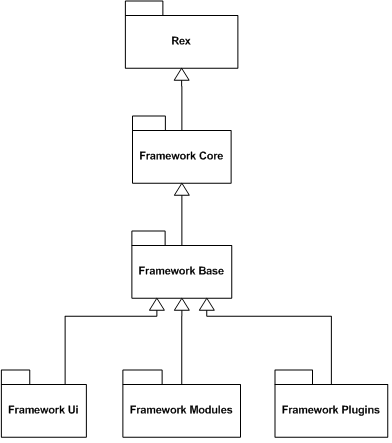
\includegraphics[height=4in,width=4in]{dev_guide_arch_packages}
\caption{Framework 3.0 package dependencies} \label{fig-arch-pkg}
\end{center}
\end{figure}

\chapter{Rex}

\par
The \textit{Rex} library is a collection of classes and modules that
may be useful to more than one project.  The most useful classes
provided by the library are documented in the following subsections.

    \section{Assembly}

\par
When writing exploits it is often necessary to have to generate
assembly instructions on the fly with variable operands, such as
immediate values, registers, and so on.  To support this
requirement, the Rex library provides classes under the
\texttt{Rex::Arch} namespace that implement architecture-dependent
opcode generation routines as well as other architecture-specific
methods, like integer packing.

        \subsection{Integer packing}

\par
Packing an integer depends on the byte-ordering of the target
architecture, whether it be big endian or little endian.  The
\texttt{Rex::Arch.pack\_addr} method supports packing an integer
using the supplied architecture type (\texttt{ARCH\_XXX}) as an
indication of which byte-ordering to use.

        \subsection{Stack pointer adjustment}

\par
Some exploits require that the stack pointer be adjusted prior to
the execution of a payload that modifies the stack in order to
prevent corruption of the payload itself.  To support this, the
\texttt{Rex::Arch.adjust\_stack\_pointer} method provides a way to
generate the opcodes that lead to adjusting the stack pointer of a
given architecture by the supplied adjustment value.  The adjustment
value can be positive or negative.

        \subsection{Architecture-specific opcode generation}

\par
Each architecture that currently has support for dynamically
generating instruction opcodes has a class under the
\texttt{Rex::Arch} namespace, such as \texttt{Rex::Arch::X86}.  The
x86 class has support for generating \texttt{jmp}, \texttt{call},
\texttt{push}, \texttt{mov}, \texttt{add}, and \texttt{sub}
instructions.

    \section{Encoding}

\par
Encoding buffers using algorithms like XOR can sometimes be useful
outside the context of an exploit.  For that reason, the Rex library
provides a basic set of classes that implement different types of
XOR encoders, such as variable length key XOR encoders and additive
feedback XOR encoders.  These classes are used by the framework to
implement different types of basic encoders that can be used by
encoder modules.  The classes for encoding buffers can be found in
the \texttt{Rex::Encoding} namespace.

    \section{Exploitation}

\par
Often times vulnerabilities will share a common attack vector or
will require a specific order of operations in order to achieve the
end-goal of code execution.  To assist in that matter, the Rex
library has a set of classes that implement some of the common
necessities that exploits have.

        \subsection{Egghunter}

\par
In some cases the exploitation of a vulnerability may be limited by
the amount of payload space that exists in the area of the overflow.
This can sometimes prevent normal methods of exploitation from being
possible due to the inability to fit a standard payload in the
amount of room that is available.  To solve this problem, an exploit
writer can make use of an \textit{egghunting} payload that searches
the target process' address space for an egg that is prefixed to a
larger payload.  This requires that an attacker have the ability to
stick the larger payload somewhere else in memory prior to
exploitation.  In the event that an egghunter is necessary, the
\texttt{Rex::Exploitation::Egghunter} class can be used.

        \subsection{SEH record generation}

\par
One attack vector that is particularly common on the Windows
platform is what is referred to as an SEH overwrite.  When this
occurs, an SEH registration record is overwritten on the stack with
user-controlled data.  To leverage this, the handler address of the
registration record is point to an address that will either directly
or indirectly lead to control of execution flow.  To make this work,
most attackers will point the handler address at the location of a
\texttt{pop/pop/ret} instruction set somewhere in the address space.
This action returns four bytes before the location of the handler
address on the stack.  In most cases, attackers will set two of the
four bytes to be equivalent a short jump instruction that hops over
the handler address and into the payload controlled by the attacker.

\par
While the common approach works fine, there is plenty of room for
improvement.  The \texttt{Rex::Exploitation::Seh} class provides
support for generating the normal (static) SEH registration record
via the \texttt{generate\_static\_seh\_record} method.  However, it
also supports the generation of a dynamic registration record that
has a random short jump length and random padding between the end of
the registration record and the actual payload.  This can be used to
make the exploit harder to signature in an IDS environment.  The
generation of a dynamic registration record is provided by
\texttt{generate\_dynamic\_seh\_record}.  Both methods are by the
\texttt{generate\_seh\_record} method that decides which of the two
methods to use based on evasion levels.

    \section{Jobs}
    \label{rex-jobs}

\par
In some cases it is helpful to break certain tasks down into the
concept of jobs.  Jobs are simply defined as finite workitems that
have a specific task.  Using this definition, the Rex library
provides a class named \texttt{Rex::JobContainer} that provides an
interface for coordinating various jobs in a centralized manner. New
jobs can be added to the job container by calling the
\texttt{add\_job} method.  Once added, a job can be started by
issuing a call to the \texttt{start\_job} method.  At any time, a
job can be stopped by calling the \texttt{stop\_job} which will also
remove the job by calling the \texttt{remove\_job} method.

\par
For more information how the usage of these API routines, please
refer to the auto-generated documentation on Metasploit website.

    \section{Logging}

\par
The Rex library provides support for the basic logging of strings to
arbitrary log sinks, such as a flat file or a database.  The logging
interface is exposed to programmers through a set of
globally-defined methods: \texttt{dlog}, \texttt{ilog},
\texttt{wlog}, \texttt{elog}, and \texttt{rlog}.  These methods
represent debug logging, information logging, warning logging, error
logging, and raw logging respectively.  Each method can be passed a
log message, a log source (the name of the component or package that
the message came from), and a log level which is a number between
zero and three.  Log sources can be registered on the fly by
\texttt{register\_log\_source} and their log level can be set by
\texttt{set\_log\_level}.

\par
The log levels are meant to make it easy to hide verbose log
messages when they are not necessary.  The use of the three log
levels is defined below:

        \subsection{LEV\_0 - Default}

This log level is the default log level if none is specified.  It
should be used when a log message should always be displayed when
logging is enabled. Very few log messages should occur at this level
aside from necessary information logging and error/warning logging.
Debug logging at level zero is not advised.

        \subsection{LEV\_1 - Extra}

This log level should be used when extra information may be needed
to understand the cause of an error or warning message or to get
debugging information that might give clues as to why something is
happening.  This log level should be used only when information may
be useful to understanding the behavior of something at a basic
level.  This log level should not be used in an exhaustively verbose
fashion.

        \subsection{LEV\_2 - Verbose}

This log level should be used when verbose information may be needed
to analyze the behavior of the framework.  This should be the
default log level for all detailed information not falling into
LEV\_0 or LEV\_1. It is recommended that this log level be used by
default if you are unsure.

        \subsection{LEV\_3 - Insanity}

This log level should contain very verbose information about the
behavior of the framework, such as detailed information about variable
states at certain phases including, but not limited to, loop iterations,
function calls, and so on.  This log level will rarely be displayed,
but when it is the information provided should make it easy to analyze
any problem.

    \section{Post-exploitation}

\par
The rex library provides client-side implementations for some
advanced post-exploitation, such as DispatchNinja and Meterpreter.
These two post-exploitation client interfaces are designed to be
usable outside of the context of an exploit.  The \texttt{Rex::Post}
namespace provides a set of classes at its root that are meant to
act as a generalized interface to remote systems via the
post-exploitation clients, if supported.  These classes allow
programmers to write automated tools that can operate upon remote
machines in a platform-independent manner.  While it's true that
platforms may lack analogous feature sets for some actions, the
majority of the common set of actions will have functional
equivalents.

    \section{Protocols}

\par
Support for some of the more common protocols, such as HTTP and SMB,
is included in the rex library to help support the development of
protocol-specific exploits and to allow for ease of use in other
projects.  Each protocol implementation exists under the
\texttt{Rex::Proto} namespace.

        \subsection{DCERC}

\par
The rex library supports a fairly robust implementation of a subset
of the DCERPC feature-set and includes support for doing invasive
actions such as multi-context bind and packet fragmentation.  The
classes that support the DCERPC client interface can be found in the
\texttt{Rex::Proto::DCERPC} namespace.

        \subsection{HTTP}

\par
Minimal support for an HTTP client and server are provided in the
rex library.  While similar protocol class implementations are
provided both in webrick and in other areas of the ruby default
standard library set, it was deemed that the current implementations
were not well suited for general purpose use due to the existence of
blocking request parsing and other such things.  The rex-provided
HTTP library also provides classes for parsing HTTP requests and
responses.  The HTTP protocol classes can be found under the
\texttt{Rex::Proto::Http} namespace.

        \subsection{SMB}

\par
Robust support for the SMB protocol is provided by the classes in
the \texttt{Rex::Proto::SMB} namespace.  These classes support
connecting to SMB servers and performing logins and other
SMB-exposed actions like transacting a named pipe and performing
other specific commands.  The SMB classes are particularly useful
for exploits that require communicating with an SMB server.

    \section{Services}

\par
One of the limitations identified in the 2.x branch of the framework
was that it was not possible to share listeners on the local machine
when attempting to perform two different exploits that both needed
to listen on the same port.  To solve this problem, the 3.0 version
of the framework provides the concept of \textit{services} which are
registered listeners that are initialized once and then subsequently
shared by future requests to allocate the same service.  This makes
it possible to do things like have two exploits waiting for an HTTP
request on port 80 without having any sort of specific conflicts.
This is especially useful because it makes it possible to not have
to worry about firewall restrictions on outbound ports that would
normally only permit connections to port 80, thus making it possible
to try multiple client-side exploits against a host with all the
different exploit instances listening on the same port for requests.

\par
Aside from the sharing of HTTP-like services, the service subsystem
also provides a way to relay connections from a local TCP port to an
already existing stream.  This support is offered through the
\texttt{Rex::Services::LocalRelay} class.

    \section{Sockets}

\par
One of the most important features of the rex library is the set of
classes that wrapper sockets.  The socket subsystem provides an
interface for creating sockets of a given protocol using what is
referred to as a \texttt{Comm} factory class.  The purpose of the
Comm factory class is to make the underlying transport and classes
used to establish the connection for a given socket opaque.  This
makes it possible for socket connections to be established using the
local socket facilities as well as by using some sort of tunneled
socket proxying system as is the case with Meterpreter connection
pivoting.

\par
Sockets are created using the socket \texttt{Parameter} class which
is initialized either directly or through the use of a hash.  The
hash initialization of the Parameters class is much the same as
perl's socket initialization.  The hash attributes supported by the
Parameter class are documented in the constructor of the Parameter
class.

\par
There are a few different ways to create sockets.  The first way is
to simply call \texttt{Rex::Socket.create} with a hash that will be
used to create a socket of the appropriate type using the supplied
or default Comm factory class.  A second approach that can be used
is to call the \texttt{Rex::Socket::create\_param} method which
takes an initialized Parameter instance as an argument.  The
remaining approaches involve using protocol-specific factory
methods, such as \texttt{create\_tcp}, \texttt{create\_tcp\_server},
and \texttt{create\_udp}.  All three of these methods take a hash as
a parameter that is translated into a Parameter instance and passed
on for actual creation.

\par
All sockets have five major attributes that are shared in common,
though some may not always be initialized.  The first attributes
provide information about the remote host and port and are exposed
through the \texttt{peerhost} and \texttt{peerport} attributes,
respectively.  The second attributes provide information the local
host and port and are exposed through the \texttt{localhost} and
\texttt{localport} attributes, respectively.  Finally, every socket
has a hash of contextual information that was used during it's
creation which is exposed through the \texttt{context} attribute.
While most exploits will have an empty hash, some exploits may have
a hash that contains state information that can be used to track the
originator of the socket.  The framework makes use of this feature
to associate sockets with framework, exploit, and payload instances.

        \subsection{Comm classes}

\par
The \texttt{Comm} interface used in the library has one simple
method called \texttt{create} which takes a \texttt{Parameter}
instance.  The purpose of this factory approach is to provide a
location and transport independent way of creating compatible socket
object instances using a generalized factory method.  For
connections being established directly from the local box, the
\texttt{Rex::Socket::Comm::Local} class is used.  For connections be
established through another machine, a medium specific Comm factory
is used, such as the Meterpreter Comm class.

\par
The \texttt{Comm} interface also supports registered event
notification handlers for when certain things occur, like prior to
and after the creation of a new socket.  This can be used by
external projects to augment the feature set of a socket or to
change its default behavior.

        \subsection{TCP sockets}

\par
TCP sockets in the Rex library are implemented as a mixin,
\texttt{Rex::Socket::Tcp}, that extends the built-in ruby Socket
base class when the local Comm factory is used.  This mixin also
includes the \texttt{Rex::IO::Stream} and \texttt{Rex::Socket}
mixins.  For TCP servers, the \texttt{Rex::Socket::TcpServer} class
should be used.

        \subsection{SSL sockets}

\par
SSL sockets are implemented on top of the normal Rex TCP socket
mixin and makes use of the OpenSSL Ruby support.  The module used
for SSL TCP sockets is \texttt{Rex::Socket::SslTcp}.

        \subsection{Switch board routing table}

\par
One of the advancements in the 3.0 version of the framework is the
concept of a local routing table that controls which Comm factory is
used for a particular route.  The reason this is useful is for
scenarios where a box is compromised that straddles an internal
network that can't be directly reached.  By adjusting the switch
board routing table to point the local subnet through a Meterpreter
Comm running the host that straddles the network, it is possible to
force the socket library to automatically use the Meterpreter Comm
factory when anything tries to communicate with hosts on the local
subnet.  This support is implemented through the
\texttt{Rex::Socket::SwitchBoard} class.

        \subsection{Subnet walking}

\par
The \texttt{Rex::Socket::SubnetWalker} class provides a way of
enumerating all the IP addresses in a subnet as described by a
subnet address and a netmask.

    \section{Synchronization}

\par
Due to the use of multi-threading, the Rex library provides extra
classes that don't exist by default in the Ruby standard library.
These classes provide extra synchronization primitives.

        \subsection{Notification events}

\par
While Ruby does have the concept of \texttt{ConditionVariable}'s, it
lacks the complete concept of notification events.  Notification
events are used extensively on platforms like Windows.  These events
can be waited on and signaled, either permanently or temporarily.
Please refer to Microsoft's online documentation for more
information. This support is provided by the
\texttt{Rex::Sync::Event} class.

        \subsection{Reader/Writer locks}

\par
A common threading primitive is the reader/writer lock.
Reader/writer locks are used to make it possible for multiple
threads to be reading a resource concurrently while only permitting
exclusive access to one thread when write operations are necessary.
This primitive is especially useful for resources that are not
updated very often as it can drastically reduce lock contentions.
While it may be overkill to have such a synchronization primitive in
the library, it's still cool.

\par
The reader/writer lock implementation is provided by the
\texttt{Rex::ReadWriteLock} class.  To lock the resource for read,
the \texttt{lock\_read} method can be used.  To lock the resource
for write access, the \texttt{lock\_write} method can be used.

        \subsection{Reference counting}

\par
In some cases it is necessary to reference count an instance in a
synchronized fashion so that it is not cleaned up or destroyed until
the last reference is gone.  For this purpose, the \texttt{Rex::Ref}
class can be used with the \texttt{refinit} method for initializing
references to 1 and the \texttt{ref} and \texttt{deref} methods that
do what their names imply.  When the reference count drops to zero,
the \texttt{cleanup} method is called on the object instance to give
it a chance to restore things back to normal.

        \subsection{Thread-safe operations}

\par
Some of the built-in functions in Ruby are not thread safe in that
they can block other ruby threads from being scheduled in certain
conditions.  To solve this problem, the functions that have issues
have been wrappered with implementations that ensure that not all
ruby threads will block.  The specific methods that required change
were \texttt{select} and \texttt{sleep}.

\chapter{Framework Core}

\par
The framework core implements the set of classes that provide an
interface to framework modules and plugins.  The core portion of the
framework is designed by used in an instance-based approach.  This
means that the entire framework state can be contained within one
class instance thereby allowing programmers to have multiple
concurrent and separate framework instances in use at the same time
rather than forcing everything to share one singleton instance.

\par
The current major version of the framework core can be accessed
through \texttt{Msf::Framework::Major} and the minor version can be
accessed through \texttt{Msf::Framework::Minor}.  A combined version
of these two version numbers can be accessed through
\texttt{Msf::Framework::Version} or \texttt{framework.version} on an
instance level.  The current revision of the framework core
interface can be accessed through
\\\texttt{Msf::Framework::Revision}.

\par
The framework core is accessed through an instance of the
\texttt{Msf::Framework} class.  Creating an instance of the
framework is illustrated in figure \ref{fig-code-framework-create}.

\begin{figure}[h]
\begin{verbatim}

framework = Msf::Framework.new
\end{verbatim}
\caption{Creating an instance of the framework}
\label{fig-code-framework-create}
\end{figure}

\par
The framework instance itself is nothing more than a way of
connecting the different critical subsystems of the framework core,
such as module management, session management, event dispatching,
and so on.  The manner of using these subsystems will be described
in the following subsections.

    \section{DataStore}

\par
Each framework instance has an instance of the
\texttt{Msf::DataStore} class that can be accessed via
\texttt{framework.datastore}.  The purpose of the datastore in the
3.0 version of the framework is to act as a replacement for the
concept of the environment in the 2.x branch.  The datastore is
simply a hash of values that may be used either by modules or by the
framework itself to reference programmer or user controlled values.
Interacting with the datastore is illustrated in figure
\ref{fig-code-framework-datastore}.

\begin{figure}[h]
\begin{verbatim}

framework.datastore['foo'] = 'bar'

if (framework.datastore['foo'] == 'bar')
    puts "'foo' is 'bar'"
end
\end{verbatim}
\caption{Creating an instance of the framework}
\label{fig-code-framework-datastore}
\end{figure}

\par
Modules will inherit values from the framework's global datastore if
they are not found in the module's localized datastore.  This aspect
will be discussed in more detail in chapter \ref{framework-modules}.

    \section{Event Notifications}

\par
One of the major goals with the 3.0 version of the framework was to
provide developers with a useful event notification system that
would allow them to perform arbitrary actions when certain framework
events occurred.  To support this, each framework instance can have
event handlers registered through the \texttt{framework.events}
attribute which is an instance of the \texttt{Msf::EventDispatcher}
class.

\par
The \texttt{EventDispatcher} class supports registering events for a
few basic different categories.  These categories will be discussed
individually.  One of the nice aspects of the event-driven framework
is that modules can automatically indicate their interest in being
registered for event handler notifications by simply implementing
the event subscriber mixins subscribed below.  When a module is
loaded into the framework, it will automatically detect that it
includes one or more of the subscriber interfaces and automatically
register the module with the appropriate event notifiers.  This
makes it possible for modules to take certain actions when specific
events occur.

        \subsection{Exploit events}

\par
Event subscribers can be registered to be notified when events
regarding exploitation occur.  To register an exploit event
subscriber, a call should be made to
\texttt{framework.events.register\_exploit\_subscriber}.  This
method should be passed an instance of an object that includes the
\texttt{Msf::ExploitEvent} mixin.  The type of event that this
subscriber will be notified of is when an exploit succeeds.  In the
event that an exploit succeeds, the subscriber's
\texttt{on\_exploit\_success} method will be called with the exploit
instance that succeeded and the session instance that it created.

\par
To remove an event subscriber, a call should be made to\\
\texttt{framework.events.remove\_exploit\_subscriber} passing the
object instance that was used to add the subscriber in the first
place.

        \subsection{General framework events}

\par
To receive event notifications about internal framework events, a
general event subscriber can be registered through the
\texttt{framework.events.register\_general\_subscriber} method.
This method takes an instance of an object that includes the
\texttt{Msf::GeneralEventSubscriber} mixin.  When a module is loaded
into the framework instance, the \texttt{on\_module\_load\_proc}
will be called if it is non-nil and will be passed the reference
name and class associated with the newly loaded module. When a
module instance is created, the \texttt{on\_module\_created\_proc}
will be called if it's non-nil and will be passed the newly created
module instance.

\par
To remove an event subscriber, a call should be made to\\
\texttt{framework.events.remove\_general\_subscriber} passing the
object instance that was used to add the subscriber in the first
place.

        \subsection{Recon events}

\par
To receive notifications about reconnaissance events, such as when a
new host or service is detected, a recon event subscriber can be
registered through the
\texttt{framework.events.add\_recon\_subscriber} method.  This
method takes an instance of an object that implements one or both of
the \texttt{Msf::ReconEvent::HostSubscriber} or
\texttt{Msf::ReconEvent::ServiceSubscriber} mixins.  When a new host
is detected or an attribute of a host has changed, a call will be
made to the event subscriber's \texttt{on\_host\_changed} method
assuming it implements the \texttt{Msf::ReconEvent::HostSubscriber}
mixin.  When a new service is detected or an attribute of a service
has changed, a call will be made to the event subscriber's
\texttt{on\_service\_changed} method assuming it implements the
\texttt{Msf::ReconEvent::ServiceSubscriber} mixin.

\par
To remove an event subscriber, a call should be made to\\
\texttt{framework.events.remove\_recon\_subscriber} passing the
object instance that was used to add the subscriber in the first
place.

        \subsection{Session events}

\par
To receive notifications about events pertaining to sessions, a
session event subscriber can be registered through the
\texttt{framework.events.add\_session\_subscriber} method.  This
method takes an instance of an object that implements the
\texttt{Msf::SessionEvent} mixin.  When a new session is opened, the
framework will call into the subscriber's \texttt{on\_session\_open}
method with the session instance that has just been opened as the
first argument.  When a session terminates, the framework will call
into the subscriber's \texttt{on\_session\_close} method with the
session instance that is being closed.

\par
To remove an event subscriber, a call should be made to\\
\texttt{framework.events.remove\_session\_subscriber} passing the
object instance that was used to add the subscriber in the first
place.

    \section{Framework Managers}

\par
The framework core itself is composed of a few different managers
that are responsible for some of the basic aspects of the framework,
such as module and plugin management.  These managers will be
described individually.

        \subsection{Module management}

\par
The module management aspect of the framework is one of its most
integral parts.  The \texttt{Msf::ModuleManager} class is
responsible for providing the interface for loading modules and for
acting as a factory for module instance creation.  The module
manager itself can be accessed through the
\texttt{framework.modules} attribute.  The loading of modules is
accomplished by adding a search path to the module manager by making
a call to the \texttt{add\_module\_path} method.  This method will
automatically load all of the modules found within the supplied
directory\footnote{The module path must conform to the standard
module directory layout, with the base directory structure appearing
similar to the \texttt{modules} sub-directory in the framework
distribution}.

\par
Modules are symbolically identified by what is referred to as a
\textit{reference name}.  The reference name takes a form that is
similar to a directory path and is partially controlled by the
filesystem path that the module is loaded from.  An example of a
reference name would be an exploit labeled
\texttt{windows/ftp/wsftpd}.  This would mean that the exploit was
loaded from \texttt{exploits/windows/ftp/wsftpd.rb}.  It is
important to note that module's must retain a namespace hierarchy
that mirrors the path in which they are located.  For instance, the
example described previously would have the class declared as
\texttt{Msf::Exploits::Windows::Ftp::Wsftpd}.  This is necessary so
that the framework's module manager knows what namespace to look in
to see what class was added after loading the file.  The reference
name of a module can be accessed through the \texttt{refname}
attribute on both the class of the module and its instances.

\par
In order to help solve the potential for module name ambiguities
across module types, modules can also be referenced by what is
called a \textit{full reference name}.  This name is the same as the
reference name of the module but is prefixed with the module's type.
For instance, the exploit \texttt{windows/ftp/wsftpd} would become
\texttt{exploit/windows/ftp/wsftpd}.  The full reference named can
be accessed through the \texttt{fullname} attribute on both the
class of the module and its instances.

\par
In order to make the module manager easy to use, each different
module type is broken down into a more basic class called a module
set which is implemented by the \texttt{Msf::ModuleSet} class.  The
purpose of a module set is to act as a localized factory for each
different module type (exploit, encoder, nop, etc).  Each module
type-specific module set can be accessed through either
\texttt{framework.type} or \texttt{framework.modules.type}.  For
example, if one wanted to enumerate exploit modules, they would use
the \texttt{framework.exploits} method to get access to the exploit
module set.

\par
Module sets are implemented in the form of a hash that associates
the reference names of modules with their underlying classes.  To
create an instance of a module, a call is made to the module set's
\texttt{create} method passing the reference name of the module that
should be instantiated.  For example, to create an instance of an
exploit named \texttt{windows/ftp/wsftpd}, a call would be made as
shown in figure \ref{fig-code-framework-modcreate}

\begin{figure}[h]
\begin{verbatim}
framework.exploits.create('windows/ftp/wsftpd')
\end{verbatim}
\caption{Creating an instance of a framework module}
\label{fig-code-framework-modcreate}
\end{figure}

\par
The table shown in figure \ref{fig-table-modulsets} shows the
relation between module types and framework module set accessors.

\begin{figure}[h]
\begin{center}
\begin{tabular}{|l|l|}
\hline
\textbf{Module Type} & \textbf{Accessor} \\
\hline
MODULE\_ENCODER & framework.encoders \\
MODULE\_EXPLOIT & framework.exploits \\
MODULE\_NOP & framework.nops \\
MODULE\_RECON & framework.recon \\
MODULE\_PAYLOAD & framework.payloads \\
\hline
\end{tabular}
\caption{Module types and their framework accessors}
\label{fig-table-modulsets}
\end{center}
\end{figure}

\par
To reload the contents of a module, a call can be issued to
\texttt{reload\_module} passing the module instance that should be
reloaded.  This will lead to the framework re-reading the contents
of the module's underlying file path and automatically creating a
new instance of the module.

        \subsection{Plugin management}

\par
One of the new features in the 3.0 version of the framework is the
concept of framework plugins.  Unlike modules, framework plugins are
meant to add features to the framework or to change the behavior of
existing aspects of the framework.  Plugins have a very loose
definition in terms of the scope in which they can operate.  For
instance, a plugin could add an entirely new module type for use by
the framework.  Alternatively, a plugin could add commands to the
existing user interfaces that interact with the framework.  A plugin
could also register custom event subscribers for doing things like
automatically causing Meterpreter to list the contents of a
computer's C drive when a new Meterpreter session is created.  The
possibilities, as they say, are endless.

\par
The plugin manager can be accessed through the
\texttt{framework.plugins} accessor which is an instance of the
\texttt{Msf::PluginManager} class. To load a plugin, a call can be
made to \texttt{framework.plugins.load} with the path of the plugin
that is to be loaded.  Optionally, a second parameter can be passed
to the \texttt{load} method that is a hash of option parameters that
may be useful to the plugin, such as \texttt{LocalInput} and
\texttt{LocalOutput} handles for use with printing strings to the
screen or whatever medium is currently being used.  The table shown
in figure \ref{fig-table-plugin-hash} shows the pre-defined hash
elements that can be passed in the option hash.

\begin{figure}[h]
\begin{center}
\begin{tabular}{|l|p{3.5in}|}
\hline
\textbf{Hash Element} & \textbf{Description} \\
\hline
LocalInput & The local input class instance which implements the \texttt{Rex::Ui::Text::Input} interface. \\
\hline
LocalOutput & The local input class instance which implements the \texttt{Rex::Ui::Output} interface. \\
\hline
ConsoleDriver & The console driver instance of \texttt{Msf::Ui::Console::Driver}. \\
\hline
WebDriver & The console driver instance of \texttt{Msf::Ui::Web::Driver}. \\
\hline
\end{tabular}
\caption{Plugin optional constructor hash elements}
\label{fig-table-plugin-hash}
\end{center}
\end{figure}

\par
All plugins are reference counted.  This is to make it possible to
implement singleton plugins that could possibly be loaded more than
once but will only have one underlying instance.  The reference
count to an instance of a plugin is automatically incremented each
time \texttt{load} is called on it.

\par
To unload a framework plugin, a call can be made to
\texttt{framework.plugins.unload} passing the instance of the plugin
previously loaded as the first parameter.  Since all plugins are
reference counted, a plugin will not actually be unloaded until its
reference count drops to zero.

\par
For more detail on the implementation of framework plugins, please
see chapter \ref{framework-plugins}.

        \subsection{Recon management}

\par
The reconnaissance manager is used to provide an interface for
reporting information about hosts, services, and other
reconnaissance entities.  These reports are tracked internally by
the recon manager which is implemented by the
\texttt{Msf::ReconManager} class.  The recon manager can be accessed
through the \texttt{framework.reconmgr} accessor.

\par
This area of the framework is currently undergoing design review and
therefore does not have any documentation at this time.

        \subsection{Session management}

\par
The session manager is used to track sessions created from within a
framework instance as the result of an exploit succeeding.  The
purpose of sessions is to expose features to a programmer that allow
it to be interacted with.  For instance, a command shell session
allows programmers to send commands and read responses to those
commands through a well-defined API.  For more information on
sessions and how they can be interacted with, please see chapter
\ref{framework-sessions}.  The session manager itself can be
accessed through the \texttt{framework.sessions} accessor and is an
instance of the \texttt{Msf::SessionManager} class.

\par
The primary purpose of the session manager is to provide an
interface for registering new sessions and assigning them a unique
session identifier as well as allowing sessions to be deregistered
when they are destroyed.  The registering of sessions with the
framework session manager is accomplished by making a call into the
\texttt{framework.sessions.register} method which takes an instance
of a session as its argument.  This method will assign the session a
unique session identifier and add it to the managed hash of
sessions.  Sessions can be enumerated by making a call into
\texttt{framework.sessions.each\_sorted} or by calling any of the
hash-compatible enumeration methods.  To obtain the session instance
associated with a particular session identifier, the
\texttt{framework.sessions.get} method can be called with the
session identifier to look up.  When a session is being destroyed, a
call must be made to \texttt{framework.sessions.deregister} passing
the instance of the session being destroyed as the first argument.

        \subsection{Job management}

\par
Each framework instance supports running various tasks in the
context of worker threads through the concept of jobs.  The job
interface can be accessed through the \texttt{framework.jobs}
accessor which is an instance of the \texttt{Rex::JobContainer}
class.  For more information on jobs, please refer to the job
explanation in the Rex documentation in section \ref{rex-jobs}.

    \section{Utility Classes}

\par
Some classes in the framework core are intended to be used to make
certain tasks simpler without being out of scope of the core aspects
of the framework.  These classes are described below.

        \subsection{Exploit driver}

\par
The \texttt{Msf::ExploitDriver} class encapsulates the task of
running an exploit module in terms of coordinating the validation of
required module options, the validation of target selection, the
generation of a selected payload, and the execution of exploit and
payload setup and cleanup.  These operations are what has to be
performed when attempting to execute an exploit.

\par
An instance of an exploit driver is initialized as described in
figure \ref{fig-code-exploit-driver}.

\begin{figure}[h]
\begin{verbatim}
driver = Msf::ExploitDriver.new(framework)

driver.payload = payload_instance
driver.exploit = exploit_instance
driver.target_idx = 0

session = driver.run
\end{verbatim}
\caption{Using the ExploitDriver class}
\label{fig-code-exploit-driver}
\end{figure}

\par
When the \texttt{run} method is called, the first step is to
validate the options required by the payload and the exploit that
have been selected.  This is done by calling the public
\texttt{validate} method on the exploit driver instance.  In the
event that options fail to validate or that a target index has not
been properly selected, an exception will be thrown to the caller.
After validation has completed, the exploit's \texttt{TARGET} data
store element is set to the selected target index.  From there, an
encoded version of the payload is generated by calling
\texttt{generate\_payload} on the exploit instance.  Once completed,
the exploit is set up by calling \texttt{setup} on the exploit
module instance and finally the actual exploit code is triggered by
calling \texttt{exploit} on the exploit module instance.

\par
Once exploitation has completed, the exploit driver calls the
\texttt{stop\_handler} method on the payload module instance and
then calls the \texttt{cleanup} method on the exploit module
instance.

\par
The exploit driver can also be instructed to run the exploit in the
context of a job.  When this is done, the underlying exploitation
operation is done in the context of a job worker thread by calling
\texttt{framework.jobs.start\_bj\_job}.  The exploit driver can be
told to use a job by setting the \texttt{use\_job} attribute to
true.

        \subsection{Encoded payload}

\par
The purpose of the \texttt{Msf::EncodedPayload} class is to
encapsulate the operation of encoding a payload with an arbitrary
set of requirements.  To generate an encoded payload, an instance of
an \texttt{Msf::EncodedPayload} class must be created by passing its
constructor an instance of a payload as well as an optional hash of
requirements that will be used during the generation phase.  This
can be accomplished by calling the class' \texttt{create} method as
shown in figure \ref{fig-code-enc-payload}.


\begin{figure}[h]
\begin{verbatim}

encoded = Msf::EncodedPayload.create(payload_instance,
    'BadChars'      => "\x0a\0xd",
    'Space'         => 400,
    'Prepend'       => "\x41\x41",
    'Append'        => "\xcc\xcc\",
    'SaveRegisters' => "edi",
    'MinNops'       => 16)
\end{verbatim}
\caption{Creating an instance of an EncodedPayload}
\label{fig-code-exploit-driver}
\end{figure}

\par
Once an encoded payload instance has been created, the next step is
to make a call to the instance's \texttt{generate} method which will
return the encoded version of the payload.  After generation has
occurred, the following attributes can be accessed on the encoded
payload instance in order to get information about the now-encoded
payload.  Figure \ref{fig-table-enc-payload} shows the attributes
and their purposes.

\begin{figure}[h]
\begin{center}
\begin{tabular}{|l|p{3.5in}|}
\hline
\textbf{Attribute} & \textbf{Description} \\
\hline
raw & The un-encoded raw payload buffer. \\
\hline
encoded & The encoded payload buffer which may be equal to raw if no encoder was used. \\
\hline
nop\_sled\_size & The size of the NOP sled prepended to the encoded payload.  Zero if no NOPs were generated. \\
\hline
nop\_sled & The NOP sled portion of the encoded payload, if any. \\
\hline encoder & The encoder module instance that was used to encode
the
payload. \\
\hline nop & The nop module instance that was used to generate the
NOP
sled, if any. \\
\hline
\end{tabular}
\caption{\texttt{Msf::EncodedPayload} instance attributes}
\label{fig-table-enc-payload}
\end{center}
\end{figure}

\par
To control the behavior of the encoded payload class, an optional
hash can be passed into the constructor.  The table in figure
\ref{fig-table-enc-payload-options} describes the options that can
be specified and the affect they have on behavior.


\begin{figure}[h]
\begin{center}
\begin{tabular}{|l|p{3.5in}|}
\hline
\textbf{Hash Element} & \textbf{Description} \\
\hline
BadChars & A string of bad characters to avoid when encoding. \\
\hline
Encoder & The name of the preferred encoder to use. \\
\hline
MinNops & The minimum number of NOPs to generate. \\
\hline
MaxNops & The maximum number of NOPs to generate. \\
\hline
Space & The amount of room left for use by the payload.  If this value is not specified, then NOP padding will not be performed and there will be no restrictions on payload size. \\
\hline
SaveRegisters & A white-space separated list of registers to save when generating the NOP sled. \\
\hline
Prepend & Raw instructions or text to prepend to the encoded payload. \\
\hline
Append & Raw instructions or text to append to the encoded payload. \\
\hline
\end{tabular}
\caption{\texttt{Msf::EncodedPayload} constructor options}
\label{fig-table-enc-payload-options}
\end{center}
\end{figure}

\chapter{Framework Base}

\par
The framework base is a library layer built on top of the framework
core that adds classes that make dealing with the framework easier.
It also provides a set of classes that could be useful to third
party development tools that don't necessarily fit within the scope
of the framework core itself.  The classes that compose the
framework base are described in the following subsections.

    \section{Configuration}

\par
One important aspect of a managed framework installation is the
concept of persistent configuration and methods for getting
information about the structure of an installation, such as the root
directory of the installation and other types of attributes.  To
facilitate this, the framework base library provides the
\texttt{Msf::Config} class that has methods for obtaining various
installation directories.  It also supports the serialization of
configuration files.  The table shown in figure
\ref{fig-table-config} describes the different methods that can be
used to obtain configuration information.


\begin{figure}[h]
\begin{center}
\begin{tabular}{|l|p{3.5in}|}
\hline
\textbf{Method} & \textbf{Description} \\
\hline
install\_root & The installation's root directory. \\
\hline
config\_directory & The configuration directory (\verb#~/.msf3#). \\
\hline
module\_directory & install\_root + '/modules'. \\
\hline
plugin\_directory & install\_root + '/plugins'. \\
\hline
log\_directory & config\_directory + '/logs'. \\
\hline
session\_log\_directory & config\_directory + '/logs/sessions'. \\
\hline
user\_module\_directory & config\_directory + '/modules'. \\
\hline
data\_directory & install\_root + '/data'. \\
\hline
config\_file & config\_directory + '/config'. \\
\hline
load & Loads the contents of a configuration file and returns an instance of a \texttt{Rex::Parser::Ini} object. \\
\hline
save & Saves the supplied option hash to the configuration file supplied as \texttt{'ConfigFile'} in the options hash or the config\_file by default. \\
\hline
\end{tabular}
\caption{\texttt{Msf::Config} accessor methods}
\label{fig-table-config}
\end{center}
\end{figure}

    \section{Logging}

\par
The framework base library provides a wrapper class that can be used
to control debug logging at an administrative level by providing
methods for enabling log sources and for controlling logs that are
applied to sessions created from within a framework instance.  To
initialize logging, a call must be made to
\texttt{Msf::Logging.init} which will register the log sources
\texttt{rex}, \texttt{core}, and \texttt{base} as being directory at
\texttt{framework.log} as found in the
\texttt{Msf::Config.log\_directory}.  Individual log sources can be
subsequently enabled or disabled by making calls to
\texttt{Msf::Logging.enable\_log\_source} and
\texttt{Msf::Logging.disable\_log\_source}, respectively.  When
session logging is enabled, calls can be issued to
\texttt{start\_session\_log} and \texttt{stop\_session\_log} which
operate on a provided session to start or stop logging to a
session-specific log file in the
\texttt{Msf::Config.session\_log\_directory} directory.

    \section{Serialization}

\par
To make life easier for framework programmer's, the framework base
library provides a class that can be used to serialize information
about modules, such as their description, options, and other
information to a uniform, human readable format.  The class that
provides this feature is the \texttt{Msf::Serializer::ReadableText}
class.  For more information, please review the auto-generated API
documentation on the Metasploit website.

    \section{Sessions}

\par
While the framework core has an abstract concept of sessions as
described through the \texttt{Msf::Session} base module, the
framework base actually provides some of the concrete
implementations.  This separation was done to eliminate
module-specific session implementations from the framework core as
the core should have no conceptual dependencies on modules that use
it where as the base library is more of a facilitation layer for
subscribers of the framework.  The two sessions currently
implemented in the base library are the \texttt{CommandShell}
session and the \texttt{Meterpreter} session.

        \subsection{CommandShell}

\par
The command shell session implements the framework core \\
\texttt{Msf::Session::Provider::SingleCommandShell} interface
against a connected stream, such as a TCP connection.  For more
information about this mixin, please read chapter
\ref{framework-sessions}.

        \subsection{Meterpreter}

\par
The meterpreter session implements the
\texttt{Msf::Session::Interactive} and \\
\texttt{Msf::Session::Comm}
mixins.  This allows it to be operated through an interactive user
shell and also indicates to the framework that internet traffic can
be routed (pivoted) through the session by making use of it as a
Comm socket factory.  The session itself is merely an extension of
the \texttt{Rex::Post::Meterpreter} class which operates against a
connected stream, such as a TCP connection.

    \section{Simplified Framework}

\par
The simplified framework provides methods that make the framework
and the different module types easier to use by providing wrapper
methods that handle most of the actions that would be common to a
subscriber of the framework.  To create an instance of the
simplified framework, the \texttt{Msf::Simple::Framework.create}
method should be called along with an optional hash.  The return
value is an instance of an \texttt{Msf::Framework} class that has
been extended by the \texttt{Msf::Simple::Framework} mixin. Existing
framework instances can also be simplified by calling the
\texttt{Msf::Simple::Framework.simplify} method with the existing
framework instance as the first argument.

\par
The creation of a simplified framework instance automatically leads
to the initialization of the \texttt{Msf::Config} class and the
\texttt{Msf::Logging} class.  Any existing configuration file is
also automatically loaded.  The default global module directory
(\texttt{Msf::Config::module\_directory} and the user-specific
module directory (\texttt{Msf::Config::user\_module\_directory} are
added as search paths to the framework instance which leads to the
loading of all modules within the two directories.  Finally, a
general event subscriber is registered with the framework instance
that will be called whenever module instances are created within the
framework.  This allows the simplified framework the opportunity to
simplify each created module instance.

\par
Each module type has a simplified framework module mixin that is
automatically used to extend created module instances via the
general event subscriber described above.  For example, when an
exploit module instance is created, the instance is extended by the
\texttt{Msf::Simple::Exploit} mixin.  Each different module mixin
provides a helper method or methods for driver that specific module
type's primary action or actions.  Furthermore, each module instance
has methods that can be used to save and restore module-specific
configuration elements through the \texttt{save\_config} and
\texttt{load\_config} methods.  Each module-specific mixin is
described individually below.

        \subsection{Exploit}

\par
The simplified exploit mixin provided in
\texttt{Msf::Simple::Exploit} extends each exploit module instance
with a method called \texttt{exploit\_simple}.  This method takes a
hash parameter that is used to control the exploitation of something
by creating an instance of an \texttt{Msf::ExploitDriver} class and
doing all the required initialization and configuration of the
module prior to issuing the call to the exploit driver's
\texttt{run} method.  If the operation succeeds, the return value is
a session instance.  Otherwise, an exception will be thrown.  For
more information about the hash elements that can be passed in,
please refer to the auto-generated API documentation on the
Metasploit website.

        \subsection{NOP}

\par
The simplified NOP mixin provided in \texttt{Msf::Simple::Nop}
extends each nop module instance with a method called
\texttt{generate\_simple}.  This method takes the length of the sled
generate and the hash of options that should be used for the
generation.  On success, the return value is a buffer that is
encoded using the \texttt{Msf::Simple::Buffer} class using the
format specified in the option hash as the \texttt{'Format'}
element.  If no format is specified, the raw version of the NOP sled
is returned.

        \subsection{Payload}

\par
The simplified payload mixin provided in
\texttt{Msf::Simple::Payload} extends each payload module instance
with a method called \texttt{generate\_simple}.  This method takes a
hash of options that are used to generate a payload buffer.  The
elements that can be used in the option hash can be found in the
auto-generated API documentation found on the Metasploit website. If
the operation is successful, the encoded payload buffer will be
serialized to the format supplied in the \texttt{'Format'} hash
element.  If the format is not raw, any staged payloads will also be
appended to the serialized buffer.

        \subsection{Recon}

\par
The reconnaissance interface is under design review.

\chapter{Framework Ui}
    \section{Console}
    \section{Web}
\chapter{Framework Modules}
\label{framework-modules}

    \section{Encoder}
    \section{Exploit}
        \subsection{Stances}
        \subsection{Types}
        \subsection{Mixins}
    \section{Nop}
    \section{Payload}
        \subsection{Single}
        \subsection{Stage}
        \subsection{Stager}
    \section{Recon}
        \subsection{Discovery}
        \subsection{Analyzer}
\chapter{Framework Plugins}
\label{framework-plugins}

    \section{User-interface Plugins}
\chapter{Framework Sessions}
\label{framework-sessions}
    \section{Command Shell}
    \section{Meterpreter}
\chapter{Methodologies}
    \section{Writing an Exploit}
\chapter{Conclusion}

\end{document}
